\documentclass[10pt,letterpaper]{article}
\usepackage{fullpage}
\usepackage[top=2cm, bottom=4.5cm, left=2.5cm, right=2.5cm]{geometry}
\usepackage{amsmath,amsthm,amsfonts,amssymb,amscd}
\usepackage{lastpage}
\usepackage{enumerate}
\usepackage{fancyhdr}
\usepackage{mathrsfs}
\usepackage{xcolor}
\usepackage{graphicx}
\usepackage{listings}
\usepackage{hyperref}

\hypersetup{%
  colorlinks=true,
  linkcolor=blue,
  linkbordercolor={0 0 1}
}
 
\renewcommand\lstlistingname{Algorithm}
\renewcommand\lstlistlistingname{Algorithms}
\def\lstlistingautorefname{Alg.}

\lstdefinestyle{Python}{
    language        = Python,
    frame           = lines, 
    basicstyle      = \footnotesize,
    keywordstyle    = \color{blue},
    stringstyle     = \color{green},
    commentstyle    = \color{red}\ttfamily
}

\setlength{\parindent}{0.0in}
\setlength{\parskip}{0.05in}
\begin{document}






Foundations of Applied Math\\
 HW \#9\\
 Due Friday, Nov. 13 by 7 am
 
\textbf{Reminder} You need to turn in a .zipped folder that contains your .tex file, your image files, your python files  and the tex file must compile.
Rename the .tex file: HW9$\_$YourLastName.tex and call the folder which you will compress: HW9$\_$YourLastName


\begin{enumerate}

\item Given $y=4x$, find an approximation to the average value of $y$ for $x \in [0,2]$.
Please do this by evaluating $y$ at 1000 randomly chosen $x$ values and average the results.\\
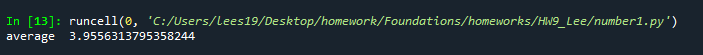
\includegraphics[scale = .8]{number1.png}\\
number1.py is included.

\item 
\begin{enumerate}[a)]
\item 
Compute $\frac{1}{2-0}\int_0^2 4x dx$- recall we have a python command to compute a definite integral that we learned about on Nov. 5.
\\

\includegraphics[scale = .8]{number2a.png}\\
number2a.py is included.
\item How does this number relate to your answer that you found in the previous problem? Why would this be the case?
\\
The numbers are very similar. This is because we are choosing random points on the line 
and averaging them so we expect the average of our random points to be around $4$. 

\end{enumerate}
\item Explain every line of this program  at the link below is doing and what this program is doing. Feel free to change items to smaller parameters to help you understand what each line is doing:

{\tiny \url{https://scipy-lectures.org/intro/numpy/auto_examples/plot_randomwalk.html#sphx-glr-intro-numpy-auto-examples-plot-randomwalk-py}}
\\
First, we import numpy and matplotlib.pyplot. Then we make variables $n_stories$, $t_max$, 
t and set them as 1000, 200, and an array from 0 to 199. Then we will create steps 
which is going to be a matrix which is $(1000, 200)$ and filled with steps of size 
$1$ or $-1$. Then we will use that matrix to create positions, which will count up 
each step for each of our realizations. $Sq_distance$ will square everything 
in positions and $mean_sq_distance$ will average all of the square values by column
so we get a $(200,)$ matrix which has the average square distance for amount of 
steps taken. plt.figure(figsize = (4, 3)) will set the size of the plot that shows
up, plt.plot will plot the distance from the origin as a function of time and compare 
it with the theoretical result. plt.xlabel and plt.ylabel will create $x$ and $y$ 
labels respectively. $plt.tight_layout()$ seems to fit the correct axes together on 
the plot. plot.show() shows the plot. 

 \item  Suppose we wish to write a Monte Carlo program that returns an estimate of the volume under $z=25-x^2-y^2$ and above the $xy$-plane.
 \begin{enumerate}[a)]
\item  Find the equation of the curve of intersection between $z=25-x^2-y^2$ and the $xy$-plane. (Note the $xy-$plane is where $z=0$.)
\\
Taking $z = 0$, we find that 
\begin{gather*}
  0 = 25 - x^2 - y^2 \\
  x^2 + y^2 = 25\\
\end{gather*}
So the intersection between $z = 25-x^2-y^2$ and the xy-plane is is the circle 
$x^2 + y^2 = 25$. 
\item Calculate the volume of the smallest rectangular prism that contains this solid.
\\
Since the intersection is a circle of radius five and the maximum height above the 
positive xy-plane the smallest box will be $10$ by $10$ by $25$ which has a volume of $2500$. 

\item  Write a python program that outputs an estimate of the volume of this solid.  Do this in two ways:
\begin{enumerate}
\item  Using vectorized code like we did Week 9- please time the code.

\item  Using a loop $N$ times as we spoke about in class and as the book in 5.1 uses- please time the code.
\end {enumerate}
Note. To time the code the following are the commands you will need.
\begin{lstlisting}
import time

t0 = time.time() 
#For i. have this right before the np.random.uniform(a,b,N) assignment statement 
#For ii have this right before the loop

t1=time.time() #have this at the end after the computation.
print("The total time using vectorized code this took was: ",t1-t0) 
#and write "using a loop" instead if it's for ii.
\end{lstlisting}
number4.py is included. \\
Using vectorized vs for loop code shows quite a difference in the amount of 
time it takes to estimate the volume of the paraboloid. \\
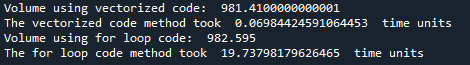
\includegraphics[scale = .8]{number4.png}

\end{enumerate}

\newpage
\item Please state whether or not the two functions {\tt randomwalk} and {\tt randomwalk2}  are equivalent below: 

 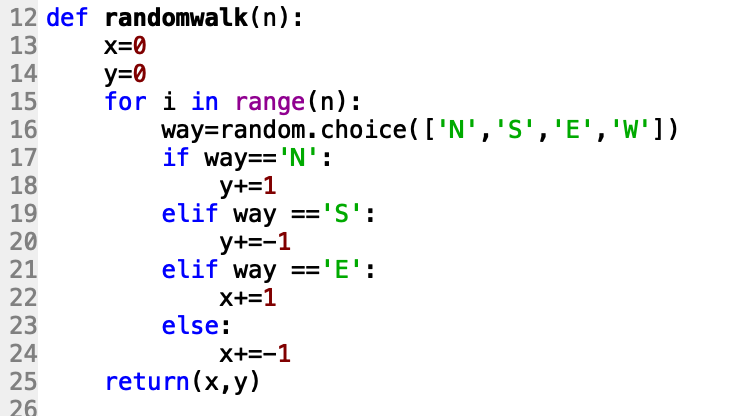
\includegraphics[scale=.5]{code2.png}  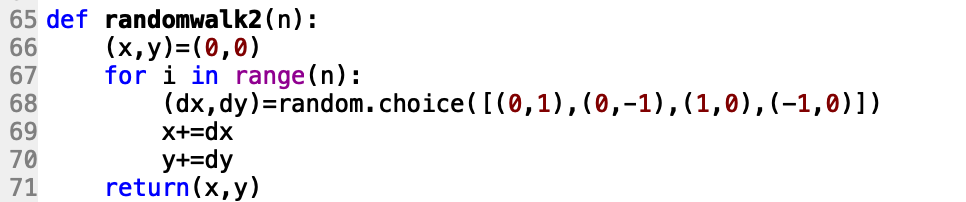
\includegraphics[scale=.5]{code.png}

Your answer must include a detailed explanation.
\\
Both methods are the same, and we can break it down into four cases.
When randomwalk chooses N, we are adding 1 to our y value, which is the same when 
randomwalk2 chooses $(0, 1)$. When randomwalk chooses S, it is the same as 
randomwalk2 choosing $(0, -1)$. When randomwalk chooses E, the equivalent in 
randomwalk2 is $(1, 0)$ and when randomwalk chooses W, the equivalent is $(-1, 0)$. 

Since all of the cases in randomwalk are covered in randomwalk2, they produce the 
same values thus they are equivalent.  
 \item Find the longest random walk which will, with probability greater than or equal to 50\%, leave you less than or equal to 5 blocks from the your starting point.
Use a Monte Carlo simulation to solve this and include your python code pasted in here and attached as a file in your zipped folder.

number6.py is included. \\
Using the Monte Carlo method, we find that the longest random walk which will leave 
you less than or equal to 5 blocks away from the start with probability greater than 
or equal to 50\% is 31 steps. 

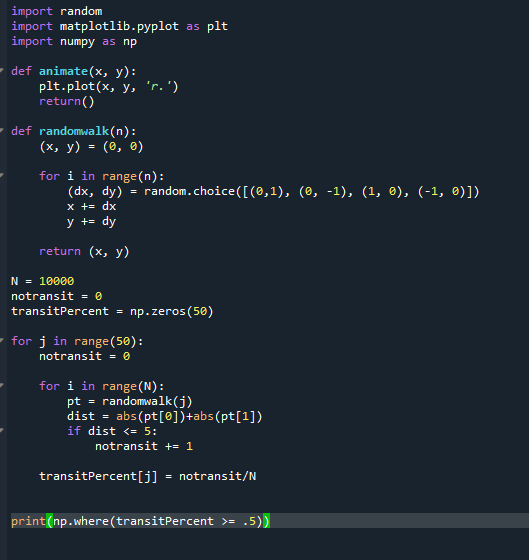
\includegraphics{number6.png}\\
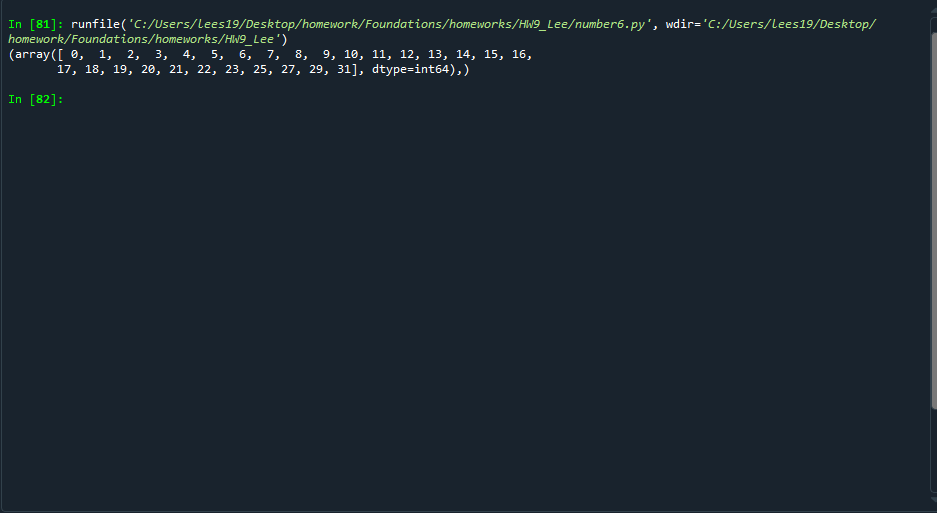
\includegraphics[scale = .7]{number6b.png}

\end{enumerate}
\end{document}